\documentclass[preview]{standalone}

\usepackage{graphicx}
\usepackage[utf8]{inputenc} %Sonderzeichen/Zeichenkodierung
\usepackage[english]{babel} %Sprache
\usepackage{amsmath, mathtools}
\usepackage{tikz}
\usepackage{subcaption}

\begin{document}
	\begin{figure}
		\centering
		\begin{subfigure}[t]{0.3\linewidth}
			\centering
			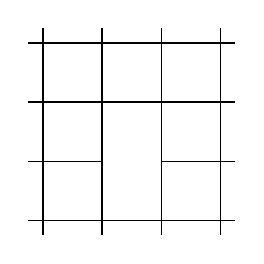
\begin{tikzpicture}[scale=0.75,baseline=(current bounding box.center)]
			%horizontal lines
			\draw (-0.25,0) -- (3.25,0);
			\draw (-0.25,-1) -- (3.25,-1);
			\draw (-0.25,-2) -- (1,-2);
			\draw (2,-2) -- (3.25,-2);
			\draw (-0.25,-3) -- (3.25,-3);
			%vertical lines
			\draw (0,-3.25) -- (0,0.25);
			\draw (1,-3.25) -- (1,0.25);
			\draw (2,-3.25) -- (2,0.25);
			\draw (3,-3.25) -- (3,0.25);
			\end{tikzpicture}
			\caption{One missing qubit defect on a toric code lattice.}
		\end{subfigure}\vspace{20pt}
		
		\begin{subfigure}[t]{0.3\linewidth}
			\centering
			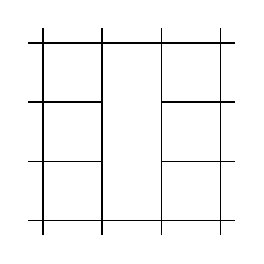
\begin{tikzpicture}[scale=0.75,baseline=(current bounding box.center)]
			%horizontal lines
			\draw (-0.25,0) -- (3.25,0);
			\draw (-0.25,-1) -- (1,-1);
			\draw (2,-1) -- (3.25,-1);
			\draw (-0.25,-2) -- (1,-2);
			\draw (2,-2) -- (3.25,-2);
			\draw (-0.25,-3) -- (3.25,-3);
			%vertical lines
			\draw (0,-3.25) -- (0,0.25);
			\draw (1,-3.25) -- (1,0.25);
			\draw (2,-3.25) -- (2,0.25);
			\draw (3,-3.25) -- (3,0.25);
			\end{tikzpicture}
			\caption{Two adjacent missing qubit defects on a toric code lattice.}
		\end{subfigure}\vspace{20pt}
		
		\begin{subfigure}[t]{0.3\linewidth}
			\centering
			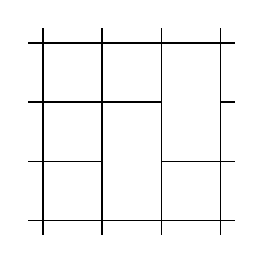
\begin{tikzpicture}[scale=0.75,baseline=(current bounding box.center)]
			%horizontal lines
			\draw (-0.25,0) -- (3.25,0);
			\draw (-0.25,-1) -- (2,-1);
			\draw (3,-1) -- (3.25,-1);
			\draw (-0.25,-2) -- (1,-2);
			\draw (2,-2) -- (3.25,-2);
			\draw (-0.25,-3) -- (3.25,-3);
			%vertical lines
			\draw (0,-3.25) -- (0,0.25);
			\draw (1,-3.25) -- (1,0.25);
			\draw (2,-3.25) -- (2,0.25);
			\draw (3,-3.25) -- (3,0.25);
			\end{tikzpicture}
			\caption{Two distant missing qubit defects on a toric code lattice.}
		\end{subfigure}
		\caption{Depiction of different situations where missing qubit defects are inserted on a toric code lattice. In the case of more than one missing link the ground space for the system depends on whether the defects are adjacent to each other.}
	\end{figure}
\end{document}